
%%%%%%%%%%%%%%%%%%%%%%% file typeinst.tex %%%%%%%%%%%%%%%%%%%%%%%%%
%
% This is the LaTeX source for the instructions to authors using
% the LaTeX document class 'llncs.cls' for contributions to
% the Lecture Notes in Computer Sciences series.
% http://www.springer.com/lncs       Springer Heidelberg 2006/05/04
%
% It may be used as a template for your own input - copy it
% to a new file with a new name and use it as the basis
% for your article.
%
% NB: the document class 'llncs' has its own and detailed documentation, see
% ftp://ftp.springer.de/data/pubftp/pub/tex/latex/llncs/latex2e/llncsdoc.pdf
%
%%%%%%%%%%%%%%%%%%%%%%%%%%%%%%%%%%%%%%%%%%%%%%%%%%%%%%%%%%%%%%%%%%%


\documentclass[runningheads,a4paper]{llncs}

\usepackage{amssymb}
\setcounter{tocdepth}{3}
\usepackage{graphicx}

\usepackage{xcolor}
\newcommand{\todo}[1]{[{\color{blue}#1}]}

\usepackage{url}
\urldef{\mailsa}\path|{alfred.hofmann, ursula.barth, ingrid.haas, frank.holzwarth,|
\urldef{\mailsb}\path|anna.kramer, leonie.kunz, christine.reiss, nicole.sator,|
\urldef{\mailsc}\path|erika.siebert-cole, peter.strasser, lncs}@springer.com|    
\newcommand{\keywords}[1]{\par\addvspace\baselineskip
\noindent\keywordname\enspace\ignorespaces#1}

\begin{document}

\mainmatter  % start of an individual contribution

% first the title is needed
\title{Object-Oriented Programming with\\Monadic State Hierarchies}

% a short form should be given in case it is too long for the running head
%\titlerunning{Programming with monadic state hierarchies}

% the name(s) of the author(s) follow(s) next
%
% NB: Chinese authors should write their first names(s) in front of
% their surnames. This ensures that the names appear correctly in
% the running heads and the author index.
%
\author{Michael B. Gale \and Alan Mycroft}
%
%\authorrunning{Lecture Notes in Computer Science: Authors' Instructions}
% (feature abused for this document to repeat the title also on left hand pages)

% the affiliations are given next; don't give your e-mail address
% unless you accept that it will be published
\institute{Computer Laboratory, University of Cambridge}

%
% NB: a more complex sample for affiliations and the mapping to the
% corresponding authors can be found in the file "llncs.dem"
% (search for the string "\mainmatter" where a contribution starts).
% "llncs.dem" accompanies the document class "llncs.cls".
%

\toctitle{Lecture Notes in Computer Science}
\tocauthor{Authors' Instructions}
\maketitle


\begin{abstract}
We present an encoding of an object system in pure Haskell which supports most conventional features of object-oriented languages, including object classes, inheritance, subtype polymorphism, and dynamic dispatch. We show a correspondence between inheritance and monad transformers by defining a state monad transformer for each class, parametrised only over the class's own state. The methods of a class are monadic computations which run on top of a stack of monad transformers, consisting of one layer for the class and each of its ancestors. The well-known limitation that functions must be ``lifted'' into the right place within a monad stack is overcome using dynamic dispatch. This encoding allows class hierarchies to be open for extension in separately-compiled modules, therefore allowing the construction of modular programs. 

\keywords{Haskell, Monad Transformers, Object-Oriented Programming}
\end{abstract}


\section{Introduction}
\label{sec:introduction}

Different programming paradigms evolve independently, but occasionally cross-pollination takes place. Features inherent to the functional paradigm have made their way into object-oriented languages such as \emph{e.g.} C\# and Java. Similarly, work to combine functional and logic programming \todo{not sure what to say about this}.

\todo{Alan: may be confusing for referees with backgrounds in either OO or FUN}
\todo{Should there be some form of introduction to monads -- in particularly the state monad? Maybe a reference to a good paper?}
\todo{write short introduction to relevant background topics -- compare with e.g. functional logic programming / OO languages being influenced by FP?}

It is folklore that dynamic dispatch can be implemented in Haskell with existential types and type classes. In the following example, a value of type $\mathit{Bird}$ is constructed by applying the $\mathit{MkBird}$ constructor to some type $a$ for which there is an instance of the $\mathit{BirdLike}$ type class:
\begin{displaymath}
\begin{array}{lcl}
\mathbf{data}~\mathit{Bird} & = & \forall a. \mathit{BirdLike}~a \Rightarrow \mathit{MkBird}~a
\end{array}
\end{displaymath}
The $\mathit{Bird}$ type effectively serves as an abstract base class. It is not possible to obtain a value of this type without some other type $a$ which implements $\mathit{BirdLike}$. Any such type can be seen as a subtype of $\mathit{Bird}$ and type-casts to the base class are possible by applying the $\mathit{MkBird}$ constructor. The type class constraint ensures that every subtype has the properties we would expect of, in this example, a bird.

This is an intriguing concept, but is often perceived as an anti-pattern \todo{cite?}. After all, why should we bother with a base class type if we can simply place a type class constraint on every function expecting bird-like arguments and avoid the $\mathit{Bird}$ type all-together?

We answer this question and show how the above concept can be elevated from a neat trick without much practical use to the foundation of an object system for purely-functional languages with a range of benefits \todo{``range of''?}. Specifically, our contributions are:
\begin{itemize}
\item We build upon the technique of using existential types combined with type classes to encode a comprehensive object system in Haskell, supporting object classes, inheritance, subtype polymorphism, and non-aliased mutation \todo{adjust this list?}. In Section \ref{sec:usage} we first show how objects in our encoding are used within a standard Haskell program, before describing the encoding itself in Section \ref{sec:encoding}.
\item Class hierarchies in our encoding are open for extension in separately-compiled modules. We thereby improve upon \emph{e.g.} open data types and functions \cite{loh2006open} which require whole program compilation.
\item \todo{Alan: monad stacks?}Monad transformers are infamous \todo{cite?} for requiring programmers to explicitly reference where in a stack of monad transformers a function should be executed. In Haskell, this is accomplished by wrapping a function in a call to $\mathit{lift}$ for every monad in the stack that should be skipped. Our system hides this boilerplate in the dynamic dispatch mechanism. 
\item In Section \ref{sec:auto}, we propose a simple notation for object classes, following the conventions of object-oriented languages, that can be used by a pre-processor to generate the corresponding encodings in Haskell.
\end{itemize}

\section{Using the Encoding}
\label{sec:usage}

Before diving into the mechanics of our encoding, let us consider a couple of \todo{adjust} examples in the notation which we introduce in detail in Section \ref{sec:auto}. 

Our notation includes three new syntactic constructs within expressions. A $\mathit{pattern} <: \mathit{name}$ statement retrieves the current value of the field whose name is given by $\mathit{name}$ and binds it to $\mathit{pattern}$. Conversely, a $\mathit{expr} >: \mathit{name}$ statement sets the value of the $\mathit{name}$ field to that of $\mathit{expr}$. Identifiers containing dots, such as $n.\mathit{insertTo}$ in the example below, invoke a method on an object -- in this case, the $\mathit{insertTo}$ method is invoked on $n$.

We begin with an implementation of OO-style linked lists, for which we define a class of list items containing values of some type $a$.
\begin{displaymath}
\begin{array}{l}
\mathbf{state}~\mathit{MListItem}~a~\mathbf{where} \\
\quad \begin{array}{lcl}
\mathbf{data}~\mathit{value} & :: & a \\
\mathbf{data}~\mathit{next}  & :: & \mathit{Maybe}~(\mathit{MListItem}~a)
\end{array}\\\\
\quad \begin{array}{lcl}
\mathit{insertTo} & :: & \mathit{MListItem}~a \to ()\\
\mathit{insertTo}~v & = & \mathbf{do} \\
\multicolumn{3}{l}{\quad \begin{array}{lcl}
\mathit{mn} & <: & \mathit{next} \\
\multicolumn{3}{l}{\mathbf{case}~\mathit{mn}~\mathbf{of}} \\
\multicolumn{3}{l}{\quad \begin{array}{lcl}
\mathit{Nothing} & \to & \mathbf{do}~\mathit{Just}~v >: \mathit{next} \\
(\mathit{Just}~n) & \to & \mathbf{do}~\mathit{Just}~(\mathit{snd}~\$~n.\mathit{insertTo}~v) >: \mathit{next}
\end{array}}
\end{array}}
\end{array}
\end{array}
\end{displaymath}
This declaration introduces a new object class $\mathit{MListItem}$ with two fields, $\mathit{value}$ and $\mathit{next}$, as well as one method named $\mathit{insertTo}$. Note that the explicit typing for this method gives it a pure type, despite having the effect of transforming an object's state. The reason for this design choice is twofold: the effectful type can be inferred from the context in which the method is defined and the corresponding monad is not given a name until we desugar the class definition. % The type of this method may initially seem confusing since we would expect it to return an updated object and the $\mathbf{do}$-notation suggests a monad. This is indeed the case, but since all methods are automatically state transformers belonging to a state monad

For convenience, we define a function to serve as a smart constructor for new $\mathit{MListItem}$ objects below. The $\mathbf{new}$ keyword, followed by the name of an object class, is used to construct the internal structure of the object:
\begin{displaymath}
\begin{array}{lcl}
\mathit{mkItem} & :: & a \to \mathit{MListItem}~a \\
\mathit{mkItem}~v & = & \mathbf{new}~\mathit{MListItem}~v~\mathit{Nothing}
\end{array}
\end{displaymath}

By setting the $\mathit{next}$ field of a $\mathit{MListItem}$ object to a value other than $\mathit{Nothing}$, elements can be added to the list. A value of $\mathit{Nothing}$ indicates the end of the list. To account for the empty list, we declare a $\mathit{MutableList}$ class which we use as the start of a linked list:
\begin{displaymath}
\begin{array}{l}
\mathbf{state}~\mathit{MList}~a~\mathbf{where} \\
\quad \begin{array}{lcl}
\mathbf{data}~\mathit{root}  & :: & \mathit{Maybe}~(\mathit{MListItem}~a)
\end{array}\\\\
\quad \begin{array}{lcl}
\mathit{insert} & :: & a \to () \\
%\mathit{insert}~v & = & \mathbf{do} \\
%\multicolumn{3}{l}{\quad \begin{array}{lcl}
%\multicolumn{3}{l}{\mathbf{let}}\\
%\multicolumn{3}{l}{\quad \mathit{item} = \mathit{mkItem}~v} \\
%\mathit{mr} & <: & \mathit{root} \\
%\multicolumn{3}{l}{\mathbf{case}~\mathit{mr}~\mathbf{of}} \\
%\multicolumn{3}{l}{\quad \begin{array}{lcl}
%\mathit{Nothing} & \to & \mathbf{do}~\mathit{Just}~\mathit{item} >: \mathit{root} \\
%(\mathit{Just}~r) & \to & \mathbf{do}~\mathit{Just}~(\mathit{snd}~\$~r.\mathit{insertTo}~\mathit{item}) >: \mathit{root}
%\end{array}}
%\end{array}}
\mathit{toList} & :: & [a]
\end{array}
\end{array}
\end{displaymath}
We omit the definitions of the $\mathit{insert}$ and $\mathit{toList}$ methods as they follow similar structures as the $\mathit{insertTo}$ method of the $\mathit{MListItem}$ class. The $\mathit{mkItem}$ function can be used to turn the value to insert into a $\mathit{MListItem}$ object. To test our construction, we define a function that, given an OO-style list of integers, inserts a few integers, and finally converts it to a functional list:
\begin{displaymath}
\begin{array}{lcl}
\mathit{test} & :: & \mathit{MList}~\mathit{Int} \to [\mathit{Int}]\\
\mathit{test}~l & = & \mathbf{let} \\
\multicolumn{3}{l}{\quad \begin{array}{lcl}
a & = & \mathit{snd}~(l.\mathit{insert}~23)\\
b & = & \mathit{snd}~(l.\mathit{insert}~16)\\
c & = & \mathit{snd}~(l.\mathit{insert}~42)\\
d & = & \mathit{snd}~(l.\mathit{insert}~24)\\
\end{array}}\\
\multicolumn{3}{l}{\mathbf{in}~\mathit{fst}~(d.\mathit{toList})}
\end{array}
\end{displaymath}
%Note that we assume that the $\mathit{MList}$ class has been extended with a $\mathit{toList}$ function which traverses the OO-style list and returns a corresponding functional list. 
Applying $\mathit{test}$ to an empty list results in the following reduction:
\begin{displaymath}
\begin{array}{cl}
 & \mathit{test}~(\mathbf{new}~\mathit{MList}~\mathit{Nothing}) \\
\Rightarrow & [23,16,42,24]
\end{array}
\end{displaymath}
Now suppose that we wish to define a class of lists which are always sorted according to some predicate. Instead of starting from scratch, we define a class $\mathit{SList}$ which derives from $\mathit{MList}$. This is indicated using a notation for inheritance borrowed from C++:

\begin{displaymath}
\begin{array}{l}
\mathbf{state}~\mathit{SList}~a : \mathit{MList}~a~\mathbf{where} \\
\quad \begin{array}{lcl}
\mathbf{data}~\mathit{pred}  & :: & a \to a \to \mathit{Bool}
\end{array}\\\\
\quad \begin{array}{lcl}
\mathit{insert} & :: & a \to ()\\
\mathit{insert}~v & = & \mathbf{do} \\
\multicolumn{3}{l}{\quad \begin{array}{lcl}
\multicolumn{3}{l}{\mathbf{let}}\\
\multicolumn{3}{l}{\quad \mathit{item} = \mathit{mkItem}~v} \\
\mathit{mr} & <: & \mathit{root} \\
\multicolumn{3}{l}{\mathbf{case}~\mathit{mr}~\mathbf{of}} \\
\multicolumn{3}{l}{\quad \begin{array}{lcl}
\mathit{Nothing} & \to & \mathbf{do}~(\mathit{Just}~\mathit{item}) >: \mathit{root} \\
(\mathit{Just}~r) & \to & \mathbf{do} \\
\multicolumn{3}{l}{\quad \begin{array}{lcl}
p & <: & \mathit{pred} \\
\mathit{Just}~(\mathit{helper}~v~p~r) & >: & \mathit{root}
\end{array}}
\end{array}}
\end{array}}
\end{array}
\end{array}
\end{displaymath}
By deriving $\mathit{SList}$ from $\mathit{MList}$, it has inherited all fields and methods of its parent. Additionally, we have added a $\mathit{pred}$ field used to store the predicate according to which the list should be sorted. We have also overriden the definition of $\mathit{insert}$ to use the $\mathit{helper}$ function whose definition is given below to insert a new item at the correct position within the list:
\begin{displaymath}
\begin{array}{lcl}
\multicolumn{3}{l}{\mathit{helper} :: a \to (a \to a \to \mathit{Bool}) \to \mathit{MutableListItem}~a \to \mathit{MutableListItem}~a} \\
\mathit{helper}~v~p~i & = & \mathbf{let} \\
\multicolumn{3}{l}{\quad \begin{array}{lcl}
\mathit{rv} & = & c.\mathit{getValue} \\
\mathit{item} & = & \mathit{mkItem}~v
\end{array}}\\
\multicolumn{3}{l}{\quad \mathbf{in}~\mathbf{if}~p~v~rv~\mathbf{then}~\mathbf{case}~c.\mathit{getNext}~\mathbf{of}} \\
\multicolumn{3}{l}{\quad \quad \begin{array}{lcl}
\mathit{Nothing} & \to & c.\mathit{setNext}~\$~\mathit{Just}~\mathit{item} \\
(\mathit{Just}~n) & \to & c.\mathit{setNext}~\$~\mathit{Just}~\$~\mathit{helper}~v~p~n 
\end{array}} \\
\multicolumn{3}{l}{\quad \mathbf{else}~\mathit{item}.\mathit{setNext}~(\mathit{Just}~c)}
\end{array}
\end{displaymath}
Applying the $\mathit{test}$ function we defined earlier to an $\mathit{SList}$ object directly is not possible. In other words, even though we consider $\mathit{SList}$ to be a subtype of $\mathit{MList}$, an explicit cast must be inserted in the form of a $\mathit{downcast}$ function:
\begin{displaymath}
\begin{array}{cl}
 & \mathit{test}~(downcast~\$~\mathbf{new}~\mathit{SList}~\mathit{Nothing}~(>)) \\
\Rightarrow & [16,23,24,42]
\end{array}
\end{displaymath}   
Evaluating this expression results in a sorted list. \todo{benefits, biggest potential criticism: a lot of complexity for little (obvious) programming gain}

\section{Encoding}
\label{sec:encoding}

Our encoding is based on the technique of combining existential types with type classes to implement dynamic dispatch, as described in Section \ref{sec:introduction}. We observe that this basic technique corresponds to an interface in the object-oriented paradigm. It has no state and does not contain any function definitions, but merely serves as a base type for types which implement the methods described by the type class constraint. Values of such types can be ``cast'' to the base type by wrapping them inside the constructor. Therefore, a notation of subtyping exists on the value level as well as on the type level.

We now show how to expand this technique to include mutable state, \todo{complete this list}. Beginning with the state, we define a single-constructor data type to store the data of each object class. For example, for the $\mathit{MList}$ class shown in Section \ref{sec:usage}, we define the following\footnote{For convention, we use a prefix underscore to indicate that a function is only used internally by the encoding.}:
\begin{displaymath}
\begin{array}{lcl}
\mathbf{data}~\mathit{MListState}~a & = & \mathit{MkMListState}~\{\\
 && \quad \_ list \_ root :: \mathit{Maybe}~(\mathit{MListItemObject~a}) \\
 && \}
\end{array}
\end{displaymath}
This data type is used as parameter for a state monad transformer from Haskell's \texttt{mtl} library \todo{cite}. If a class has no parent, as is the case with $\mathit{MList}$, then it is a transformer over the $\mathit{Identity}$ monad. If a class has a parent, such as $\mathit{SList}$, then the $\mathit{Identity}$ monad is replaced with the state monad transformer corresponding to its parent class:
\begin{displaymath}
\begin{array}{lcl}
\mathbf{type}~\mathit{MList}~a & = & \mathit{StateT}~(\mathit{MListState}~a)~\mathit{Identity} \\
\mathbf{type}~\mathit{SList}~a & = & \mathit{StateT}~(\mathit{SListState}~a)~(\mathit{MList}~a)
\end{array}
\end{displaymath}
State transformers are functions which accept an initial state as argument and return a result as well as an updated state. The state monad captures this effect and state monad transformers allow state monads to be layered on top of other monads. The resulting \emph{monad stacks} have all of their monads' effects layered on top of each other. Therefore, a stack of state monad transformers will propagate the state of each layer.

For this reason, the data type representing the state of a sub-class does not include any fields inherited from its parent(s):
\begin{displaymath}
\begin{array}{lcl}
\mathbf{data}~\mathit{SListState}~a & = & \mathit{MkSListState}~\{~ \_ slist \_ pred :: a \to a \to \mathit{Bool}~\}
\end{array}
\end{displaymath}
\todo{I am not really happy with following paragraph}
We use a multi-parameter type class together with functional dependencies \todo{cite} to represent the interface of an object class. We can further divide such an interface into groups of \emph{external} and \emph{internal} methods. Each method of an object class has a corresponding function in both groups. While both groups are part of the same type class, the internal interface is used when the call-site is a method within the same object class. The external methods can be called on objects from all other call-sites, such as \emph{e.g.} pure code. They are responsible for unfolding an object into a stack of state monad transformers, invoking the corresponding internal method on the stack, and then folding the updated state back into an object. \todo{hylomorphism?} For example, the following is a partial definition of the type class for $\mathit{MList}$: 
\begin{displaymath}
\begin{array}{l}
\mathbf{class}~\mathit{Monad}~m \Rightarrow \mathit{MListLike}~e~s~m~a \mid e \to s, s \to e~\mathbf{where} \\
\quad \begin{array}{lcl}
\mathit{\_ \mathit{get}\_\mathit{list}\_\mathit{root}} & :: & e~a \to m~(\mathit{Maybe}~(\mathit{MListItemObject~a}),e~a) \\
\mathit{insert} & :: & e~a \to a \to m~((),e~a) \\
\_\mathit{insert} & :: & a \to \mathit{StateT}~(s~a)~m~()
\end{array}
\end{array}
\end{displaymath}
%\todo{The rest of this section is only outlining the structure so far and lacks lots of details}
Each type class belonging to an object class has at least three parameters: $e$ is the type representing objects, $s$ is the data type describing the state, and $m$ is the monad \todo{I want to say context so badly} in which methods of this type class can be invoked in. Additionally, there is one type parameter for each type parameter of the object class, which is $a$ for $\mathit{MList}$.

We combine all of the above to define a data type for objects belonging to an object class. The value representation of an object is reminiscent of a functional zipper.

\begin{displaymath}
\begin{array}{lcl}
\mathbf{data}~\mathit{MListObject}~a & = & \mathit{MListData}~\{ \\ 
 & & \quad \_\mathit{list}\_\mathit{data} :: \mathit{MListState}~a\\
 & & \} \\
 & \mid & \forall s~d.\mathit{MListLike}~s~d~(\mathit{MList}~a)~a \Rightarrow \mathit{MListStart}~\{\\
 & & \quad \begin{array}{lcl}
 \_\mathit{list}\_\mathit{data} & :: & \mathit{MListState}~a, \\
 \_\mathit{list}\_\mathit{sub}  & :: & s~a
 \end{array}\\
 & & \}
\end{array}
\end{displaymath}
An $\mathit{MList}$ object has two possible states: either it is an instance of $\mathit{MList}$ or it is an instance of a sub-class of $\mathit{MList}$ which has been cast to $\mathit{MList}$.

\begin{displaymath}
\begin{array}{lcl}
\mathit{newMList} & :: & \mathit{MListObject}~a \\
\mathit{newMList} & = & \mathit{MListData}~\{~\_\mathit{list}\_\mathit{data} = \mathit{MkMListState}~\{\\ 
&& \quad \_\mathit{list}\_\mathit{root} = \mathit{Nothing}\\
&& \}~\}
\end{array}
\end{displaymath}

\begin{displaymath}
\begin{array}{l}
\mathbf{instance}~\mathit{MListLike}~\mathit{MListObject}~\mathit{MListState}~\mathit{Identity}~a~\mathbf{where} \\
\quad \begin{array}{lcl}
\mathit{insert}~(\mathit{MListData}~d)~v & = & \mathbf{do} \\
\multicolumn{3}{l}{\quad \begin{array}{lcl}
(r,d') & \leftarrow & \mathit{runStateT}~(\_\mathit{insert}~v)~d \\
\multicolumn{3}{l}{\mathit{return}~(r,\mathit{MListData}~d')}
\end{array}} \\
\mathit{insert}~(\mathit{MListStart}~d~s)~v & = & \mathbf{do} \\
\multicolumn{3}{l}{\quad \begin{array}{lcl}
((r,s'),d') & \leftarrow & \mathit{runStateT}~(\mathit{insert}~s~v)~d \\
\multicolumn{3}{l}{\mathit{return}~(r,\mathit{MListStart}~d'~s')}
\end{array}} \\
\_\mathit{insert} & = & \mathit{list}\_\mathit{insert}
\end{array}
\end{array}
\end{displaymath}

%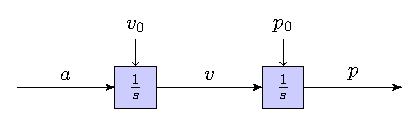
\includegraphics{images/figures-figure0.eps}

\begin{figure}
\begin{center}
\begin{tabular}{|c|c|c|c|}
\hline \emph{Base class} & None & Abstract & Final \\ 
\hline data         & x & x & x \\ 
\hline data,sub     & x & x &  \\ 
\hline sup,data     &  &  &  \\ 
\hline sup,data,sub &  &  &  \\ 
\hline 
\end{tabular} 
\end{center}
\caption{Object constructors by attribute for base classes}
\label{tab:baseconstructors}
\end{figure}

\begin{figure}
\begin{center}
\begin{tabular}{|c|c|c|c|}
\hline \emph{Sub-class} & None & Abstract & Final \\ 
\hline data         & x &   & x \\ 
\hline data,sub     & x & x &   \\ 
\hline sup,data     & x &   & x \\ 
\hline sup,data,sub & x & x &   \\ 
\hline 
\end{tabular} 
\end{center}
\caption{Object constructors by attribute for sub-classes}
\label{tab:childconstructors}
\end{figure}


\begin{itemize}
\item Different ``zipper'' arrangements depending on base/child, abstract, and final attributes
\item Type class per object class with 2 functions for each method (external vs. internal call)
\item Zipper traversal in the function definitions and construction of the monad stack
\end{itemize}

\section{Casts}
\label{sec:casts}

\todo{This section needs a better title!}

\todo{casting}

We have shown that calling a method on an object sets up a stack of state monad transformers parametrised over each $\delta$-object's state. If the object has the type of a base class, this stack can be set up in order by the dynamic dispatch mechanism. If an object has the type of a sub-class, its value representation will reflect this by having the $\delta$-object corresponding to the sub-class in view. Therefore  then this becomes more difficult.



\begin{itemize}
\item internal $\mathit{invoke}$ function which uses the zipper to construct a monad stack from an arbitrary focus
\end{itemize}

\section{Auto-generation}
\label{sec:auto}

\begin{itemize}
\item translation rules for notation to standard Haskell
\end{itemize}

\section{Related Work}
\label{sec:related}

\todo{Relevant parts from my thesis proposal:}

%Effect handlers \citep{plotkin2009handlers}, etc.

Extending Haskell with an object system is not a new idea. A previous attempt\cite{OOHaskell} presents an encoding, but focuses on remaining true to object-oriented programming. As a result, their system is impure and requires IO references to account for mutability and aliasing. \cite{shields2001object} show how to extend Haskell to allow the encoding of object-oriented style overloading. Their goal is to allow Haskell programs to provide interfaces to libraries written in object-oriented languages, but not to write object-oriented style code in Haskell itself.

In more theoretical work, \cite{Pierce93simpletype-theoretic} present a typed $\lambda$-calculus with support for encapsulation, message passing, subtyping, and inheritance. Methods in this calculus are state transformers, but they do not form stacks of state monad transformers. Instead, methods simply use the object as state as in traditional object-oriented programming.

The expression problem\cite{wadler1998expression} is concerned with extending programs with new functionality without having to change any of the existing code. A classical example of this is wishing to extend an expression language which supports basic arithmetic expressions with new forms of expressions which add \emph{e.g.} support for exceptions.  

In object-oriented programming languages this can be accomplished using an abstract class for expressions which all forms of expressions derive from. Our system allows for similar implementations. However, other approaches exist for Haskell. Open data types and functions\cite{loh2006open} is a proposed extension for Haskell which enables data types and functions to be marked as ``open''. This keyword allows new constructors and equations to be added after an initial declaration. This is accomplished by generating normal data types and functions from all open declarations within a program. This approach has the advantage that it does not introduce any new concepts to the language. However, it does require whole-program compilation and changes to the order in which pattern matching occurs.

Modular data types can be constructed in Haskell without any new extensions to Haskell's type system using the data types \`a la carte technique\cite{swierstra2008data}. This approach has been used to construct \emph{e.g.} modular compilers\cite{day2012towards}. Unlike open data types, it does not require whole-program compilation, but its barrier to entry is also higher \todo{why?}. 

\cite{jaskelioff2011monatron} shows a monad transformer library called \emph{Monatron} which features an improved lifting mechanism at the cost of increased implementation complexity. \cite{schrijvers2011monads} describe \emph{monad zippers} and \emph{monad views} which are used to hide and address parts of monad stacks, respectively.

The most promising solution so far has been presented in \cite{kiselyov2013extensible} where a single monad, parameterised over a set of effect handlers \cite{plotkin2009handlers} is used to effectively implement an effect system in Haskell. The order of effects is not fixed on the type-level, but is determined on the value level. This system is also more efficient than monad transformers since it is no longer necessary to call each monad's $\gg\!\!=$ function at every step. 

\section{Conclusion and Future Work}
\label{sec:conclusions}

We have shown how to encode an object system in pure Haskell, built on top of monad transformers. Additionally, we have proposed a notation which can be desugared. In addition to providing the advantages of the object-oriented paradigm within a functional setting, we have also seen other benefits.

The dynamic dispatch mechanism hides calls to the $\mathit{lift}$ function of monad transformers from the programmer, while also allowing more fine-grained control. Each layer of a monad stack is mapped to a corresponding class. Overriding a method in one class can be used to intercept calls from sub-classes. We believe that this is a powerful representation of monad transformers which, if generalised to monads other than the state monad, would allow us to reduce the amount of boilerplate which is currently required.

A major limitation of our encoding is the lack of aliasing. While aliasing is often considered a key feature of object-oriented programming, it requires references to an object to be shareable so that an update through one can be observed through the others -- a side effect. In impure languages, this is accomplished by storing all objects in a global heap, but this makes reasoning about such programs difficult. A good compromise may be the introduction of localised heaps which are shared between all functions which possess an alias to the same object. 

\todo{paragraph about efficient compilation}

\subsubsection*{Acknowledgments.} Content

\begin{thebibliography}{4}

\bibitem{day2012towards}
Day, Laurence~E. \& Hutton, Graham.
\newblock Towards modular compilers for effects.
\newblock In \emph{Trends in Functional Programming}, pages 49--64. Springer,
  2012.

\bibitem{jaskelioff2011monatron}
Jaskelioff, Mauro.
\newblock Monatron: An extensible monad transformer library.
\newblock In \emph{Implementation and Application of Functional Languages},
  pages 233--248. Springer, 2011.
  
\bibitem{OOHaskell}
  Kiselyov, Oleg \& L{\"a}mmel, Ralf.
  \newblock {Haskell's overlooked object system}.
  \newblock \emph{arXiv preprint cs/0509027}, 2005.
  \newblock Draft.

\bibitem{kiselyov2013extensible}
Kiselyov, Oleg \& Sabry, Amr \& Swords, Cameron.
\newblock Extensible effects: an alternative to monad transformers.
\newblock In \emph{Proceedings of the 2013 ACM SIGPLAN symposium on Haskell},
  pages 59--70. ACM, 2013.

\bibitem{loh2006open}
L{\"o}h, Andres \& Hinze, Ralf.
\newblock Open data types and open functions.
\newblock In \emph{Proceedings of the 8th ACM SIGPLAN international conference
  on Principles and practice of declarative programming}, pages 133--144. ACM,
  2006.

\bibitem{plotkin2009handlers}
Plotkin, Gordon \& Pretnar, Matija.
\newblock Handlers of algebraic effects.
\newblock In \emph{Programming Languages and Systems}, pages 80--94. Springer,
  2009.

\bibitem{schrijvers2011monads}
Schrijvers, Tom \& Oliveira, Bruno C. d.~S.
\newblock Monads, zippers and views: virtualizing the monad stack.
\newblock In \emph{ACM SIGPLAN Notices}, volume~46, pages 32--44. ACM, 2011.

\bibitem{shields2001object}
Shields, Mark \& Peyton~Jones, Simon.
\newblock Object-oriented style overloading for Haskell.
\newblock \emph{Electronic Notes in Theoretical Computer Science}, 59\penalty0
  (1):\penalty0 89--108, 2001.

\bibitem{swierstra2008data}
Swierstra, Wouter.
\newblock Data types {\`a} la carte.
\newblock \emph{Journal of functional programming}, 18\penalty0 (04):\penalty0
  423--436, 2008.

\bibitem{wadler1998expression}
Wadler, Philip.
\newblock The expression problem.
\newblock \emph{Java-genericity mailing list}, 1998.

%\bibitem{jour} Smith, T.F., Waterman, M.S.: Identification of Common Molecular
%Subsequences. J. Mol. Biol. 147, 195--197 (1981)

%\bibitem{lncschap} May, P., Ehrlich, H.C., Steinke, T.: ZIB Structure Prediction Pipeline:
%Composing a Complex Biological Workflow through Web Services. In: Nagel,
%W.E., Walter, W.V., Lehner, W. (eds.) Euro-Par 2006. LNCS, vol. 4128,
%pp. 1148--1158. Springer, Heidelberg (2006)

%\bibitem{book} Foster, I., Kesselman, C.: The Grid: Blueprint for a New Computing
%Infrastructure. Morgan Kaufmann, San Francisco (1999)

%\bibitem{proceeding1} Czajkowski, K., Fitzgerald, S., Foster, I., Kesselman, C.: Grid
%Information Services for Distributed Resource Sharing. In: 10th IEEE
%International Symposium on High Performance Distributed Computing, pp.
%181--184. IEEE Press, New York (2001)

%\bibitem{proceeding2} Foster, I., Kesselman, C., Nick, J., Tuecke, S.: The Physiology of the
%Grid: an Open Grid Services Architecture for Distributed Systems
%Integration. Technical report, Global Grid Forum (2002)

%\bibitem{url} National Center for Biotechnology Information, \url{http://www.ncbi.nlm.nih.gov}

\end{thebibliography}
\end{document}
